\documentclass[12pt, a4paper]{article}
\usepackage[utf8]{inputenc}
\usepackage{graphicx}
\usepackage{geometry}
\usepackage{amsmath}
\usepackage{hyperref}
\usepackage{float}
\usepackage{booktabs}
\usepackage{siunitx}
\usepackage{grffile}

\geometry{margin=1in}

\title{\textbf{01. Photo-electric Effect}}
\author{Yamulapalli Nandu Navadeep \\ Roll Number: IMS24267}
\date{Date of the experiment: 7 September 2026 \\ Date of Submission: \today}

\begin{document}

\maketitle


\section{Aim of the Experiment}
To determine Planck's constant ($h$) using the photoelectric effect and to study the current-voltage characteristics of the photoelectric tube under varying light intensities and frequencies.

\section{Theory}
The photoelectric effect is the emission of electrons from the surface of a metal when electromagnetic radiation shines on it. The energy of the emitted electrons is directly proportional to the frequency of the incident light. Below a certain threshold frequency, no electrons are emitted.

According to Einstein's quantum model, light consists of packets of energy called photons. The energy of a photon is given by $E = h \nu$, where $h$ is Planck's constant and $\nu$ is the frequency of light. When a photon is absorbed by an electron, part of this energy is used to overcome the work function ($W_0$) of the material, and the rest becomes the maximum kinetic energy ($KE_{max}$) of the emitted electron.
The equation is given by:
\begin{equation}
    h \nu = KE_{max} + W_0
\end{equation}

If a negative stopping potential ($V$) is applied such that even the most energetic electrons cannot reach the collector, the photocurrent becomes zero. At this point, the maximum kinetic energy is equal to the electrical potential energy:
\begin{equation}
    KE_{max} = e V
\end{equation}

Substituting this into Einstein's equation gives:
\begin{equation}
    e V = h \nu - W_0
\end{equation}
\begin{equation}
    V = \frac{h}{e} \nu - \frac{W_0}{e}
\end{equation}

This is a linear equation. Plotting the stopping potential ($V$) against frequency ($\nu$) yields a straight line with a slope of $h/e$. Planck's constant can be calculated from this slope.

\section{Procedure}
\textbf{Experiment 1: Measuring Planck's Constant}
\begin{enumerate}
    \item The mercury light source and photodiode enclosures were aligned on a track.
    \item The light source and apparatus were allowed to warm up for 10 minutes.
    \item The current amplifier was calibrated to zero.
    \item Optical filters (365 nm, 405 nm, 436 nm, 546 nm, 577 nm) were placed one by one in front of the photodiode.
    \item For each filter, the voltage was adjusted until the photocurrent became exactly zero.
    \item This stopping potential was recorded for each wavelength.
\end{enumerate}

\textbf{Experiment 2: Current Voltage Characteristics (Constant Frequency, Different Intensities)}
\begin{enumerate}
    \item A single filter (e.g., 436 nm) was used.
    \item The aperture was set to 2 mm, 4 mm, and 8 mm to change the intensity.
    \item For each aperture, the voltage was increased in small steps, and the corresponding photocurrent was recorded.
\end{enumerate}

\textbf{Experiment 3: Current Voltage Characteristics (Different Frequencies, Constant Intensity)}
\begin{enumerate}
    \item A constant aperture (e.g., 4 mm) was maintained.
    \item Different filters (365 nm, 405 nm, 436 nm) were used.
    \item For each filter, the voltage was increased in small steps, and the corresponding photocurrent was recorded.
\end{enumerate}

\section{Tabular Column}

\subsection*{Table 1: Measuring Planck's Constant ($V$ vs $f$)}
\begin{table}[H]
    \centering
    \begin{tabular}{cccccc}
        \toprule
        \textbf{Wavelength} & \textbf{Frequency} & \multicolumn{3}{c}{\textbf{Stopping Voltage (V)}} \\
        \cmidrule(lr){3-5}
        \textbf{(nm)} & \textbf{($\times 10^{14}$ Hz)} & \textbf{2 mm Aperture} & \textbf{4 mm Aperture} & \textbf{8 mm Aperture} \\
        \midrule
        365 & 8.21 & $-1.920$ & $-1.926$ & $-1.940$ \\
        405 & 7.40 & $-1.543$ & $-1.560$ & $-1.575$ \\
        436 & 6.88 & $-1.357$ & $-1.375$ & $-1.386$ \\
        546 & 5.49 & $-0.819$ & $-0.824$ & $-0.832$ \\
        577 & 5.20 & $-0.700$ & $-0.703$ & $-0.709$ \\
        \bottomrule
    \end{tabular}
    \caption{Stopping voltage measurements for different frequencies and intensities.}
\end{table}

\subsection*{Table 2: Constant Frequency, Different Intensities ($\lambda = 436$ nm)}
\begin{table}[H]
    \centering
    \begin{tabular}{cccc}
        \toprule
        \textbf{Voltage (V)} & \multicolumn{3}{c}{\textbf{Current ($\times 10^{-11}$ A)}} \\
        \cmidrule(lr){2-4}
        & \textbf{2 mm Aperture} & \textbf{4 mm Aperture} & \textbf{8 mm Aperture} \\
        \midrule
        $-4$ & 0 & 0 & 0 \\
        $-2$ & 0 & 0 & 0 \\
        $0$ & 22 & 62 & 168 \\
        $2$ & 73 & 250 & 776 \\
        $4$ & 106 & 398 & 1420 \\
        $6$ & 127 & 490 & 1800 \\
        $8$ & 147 & 570 & 2100 \\
        $10$ & 168 & 643 & 2500 \\
        $12$ & 184 & 730 & 2750 \\
        $14$ & 200 & 786 & 3000 \\
        $16$ & 216 & 843 & 3270 \\
        $18$ & 230 & 900 & 3500 \\
        $20$ & 244 & 950 & 3730 \\
        $22$ & 259 & 1006 & 3950 \\
        $24$ & 272 & 1060 & 4180 \\
        $26$ & 286 & 1124 & 4450 \\
        $28$ & 298 & 1175 & 4630 \\
        $30$ & 306 & 1225 & 4780 \\
        \bottomrule
    \end{tabular}
    \caption{Current-voltage characteristics for varying intensities at constant frequency.}
\end{table}

\subsection*{Table 3: Constant Intensity, Different Frequencies (4 mm Aperture)}
\begin{table}[H]
    \centering
    \begin{tabular}{cc|cc|cc}
        \toprule
        \multicolumn{2}{c|}{\textbf{365 nm}} & \multicolumn{2}{c|}{\textbf{405 nm}} & \multicolumn{2}{c}{\textbf{436 nm}} \\
        \textbf{Voltage (V)} & \textbf{Current ($\times 10^{-11}$ A)} & \textbf{Voltage (V)} & \textbf{Current ($\times 10^{-11}$ A)} & \textbf{Voltage (V)} & \textbf{Current ($\times 10^{-11}$ A)} \\
        \midrule
        $-1.91$ & 30 & $-0.83$ & 30 & $-0.95$ & 30 \\
        $-0.95$ & 40 & 0.11 & 60 & 0.14 & 90 \\
        0.90 & 200 & 0.94 & 100 & 0.43 & 110 \\
        1.92 & 340 & 1.32 & 120 & 0.70 & 130 \\
        2.90 & 490 & 2.12 & 170 & 1.01 & 160 \\
        3.90 & 620 & 3.12 & 220 & 1.25 & 180 \\
        4.90 & 710 & 4.12 & 250 & 1.65 & 230 \\
        5.92 & 790 & 5.12 & 280 & 1.82 & 240 \\
        7.02 & 850 & 6.12 & 300 & 1.97 & 260 \\
        7.90 & 900 & 7.15 & 330 & 2.46 & 320 \\
        8.82 & 950 & 8.16 & 340 & 2.98 & 360 \\
        9.86 & 1040 & 9.13 & 390 & 3.97 & 410 \\
        10.93 & 1080 & 10.13 & 410 & 4.96 & 460 \\
        11.97 & 1180 & 11.17 & 430 & 5.97 & 510 \\
        12.90 & 1210 & 12.10 & 440 & 6.97 & 540 \\
        13.84 & 1270 & 13.10 & 460 & 7.97 & 570 \\
        14.94 & 1290 & 14.12 & 490 & 8.96 & 610 \\
        15.97 & 1370 & 15.12 & 500 & 9.95 & 630 \\
        16.89 & 1420 & 16.14 & 520 & 10.92 & 690 \\
         &  & 17.11 & 530 & 11.92 & 720 \\
         &  & 18.14 & 570 & 12.92 & 750 \\
         &  & 19.25 & 580 & 13.92 & 790 \\
         &  &  &  & 14.93 & 850 \\
         &  &  &  & 15.93 & 870 \\
         &  &  &  & 16.93 & 880 \\
         &  &  &  & 17.93 & 900 \\
         &  &  &  & 18.93 & 930 \\
        \bottomrule
    \end{tabular}
    \caption{Current-voltage characteristics for different frequencies at constant intensity (4 mm aperture).}
\end{table}

\section{Calculations}
The photoelectric equation is given by:
\begin{equation}
    V = \frac{h}{e}\nu - \frac{W_0}{e}
\end{equation}
where $V$ is the stopping potential (taken as a positive magnitude for the plot), $\nu$ is the frequency of incident light, $h$ is Planck's constant, $e$ is the elementary charge ($1.602 \times 10^{-19}$ C), and $W_0$ is the work function.

A plot of $V$ versus $\nu$ yields a straight line with:
\begin{itemize}
    \item \textbf{Slope ($m$)} = $\frac{h}{e}$
    \item \textbf{y-intercept ($c$)} = $-\frac{W_0}{e}$
    \item \textbf{x-intercept ($\nu_0$)} = $\frac{W_0}{h}$ (Threshold Frequency)
\end{itemize}

\subsection*{Detailed Calculation for 2 mm Aperture}
From the linear fit of the data for the 2 mm aperture, the slope and y-intercept are determined as:
\begin{align*}
    m_1 &= 3.984 \times 10^{-15} \text{ V}\cdot\text{s} \\
    c_1 &= -1.376 \text{ V}
\end{align*}

\textbf{1. Planck's Constant ($h_1$):}
\begin{align*}
    h_1 &= m_1 \times e \\
    h_1 &= (3.984 \times 10^{-15} \text{ V}\cdot\text{s}) \times (1.602 \times 10^{-19} \text{ C}) \\
    h_1 &= 6.382 \times 10^{-34} \text{ J}\cdot\text{s}
\end{align*}

\textbf{2. Work Function ($W_{0,1}$):}
The y-intercept represents $-\frac{W_0}{e}$. Thus, the work function in electron-volts (eV) is the magnitude of the y-intercept:
\begin{align*}
    W_{0,1} &= -c_1 \times e \\
    W_{0,1} &= -(-1.376 \text{ V}) \times 1 \text{ e} \\
    W_{0,1} &= 1.376 \text{ eV}
\end{align*}

\textbf{3. Threshold Frequency ($\nu_{0,1}$):}
The threshold frequency is the x-intercept, where the stopping potential $V = 0$:
\begin{align*}
    \nu_{0,1} &= -\frac{c_1}{m_1} \\
    \nu_{0,1} &= \frac{1.376 \text{ V}}{3.984 \times 10^{-15} \text{ V}\cdot\text{s}} \\
    \nu_{0,1} &= 3.454 \times 10^{14} \text{ Hz}
\end{align*}

\subsection*{Summary for All Apertures}
Applying the same method to the 4 mm and 8 mm apertures yields the following:

For the 4 mm aperture:
\begin{itemize}
    \item $h_2 = 6.435 \times 10^{-34} \text{ J}\cdot\text{s}$
    \item $W_{0,2} = 1.384 \text{ eV}$
    \item $\nu_{0,2} = 3.450 \times 10^{14} \text{ Hz}$
\end{itemize}

For the 8 mm aperture:
\begin{itemize}
    \item $h_3 = 6.469 \times 10^{-34} \text{ J}\cdot\text{s}$
    \item $W_{0,3} = 1.392 \text{ eV}$
    \item $\nu_{0,3} = 3.446 \times 10^{14} \text{ Hz}$
\end{itemize}

The average values calculated from these measurements are:
\begin{align*}
    h_{avg} &= \frac{6.382 + 6.435 + 6.469}{3} \times 10^{-34} = 6.428 \times 10^{-34} \text{ J}\cdot\text{s} \\
    W_{0,avg} &= \frac{1.376 + 1.384 + 1.392}{3} = 1.384 \text{ eV} \\
    \nu_{0,avg} &= \frac{3.454 + 3.450 + 3.446}{3} \times 10^{14} = 3.450 \times 10^{14} \text{ Hz}
\end{align*}

\section{Results}
The key findings of the experiment are as follows:
\begin{itemize}
    \item The experimentally determined average value of Planck's constant is $h_{avg} = 6.428 \times 10^{-34}$ J$\cdot$s.
    \item The average work function of the photoelectric material is $W_{0,avg} = 1.384$ eV.
    \item The average threshold frequency is $\nu_{0,avg} = 3.450 \times 10^{14}$ Hz.
\end{itemize}

The current-voltage characteristics confirm that:
\begin{itemize}
    \item Saturation current increases with light intensity (aperture size), but the stopping potential remains constant for a given frequency.
    \item The stopping potential becomes more negative as the frequency of incident light increases.
\end{itemize}

\section{Graph}
The following graphs illustrate the data obtained during the experiment:

\begin{figure}[H]
    \centering
    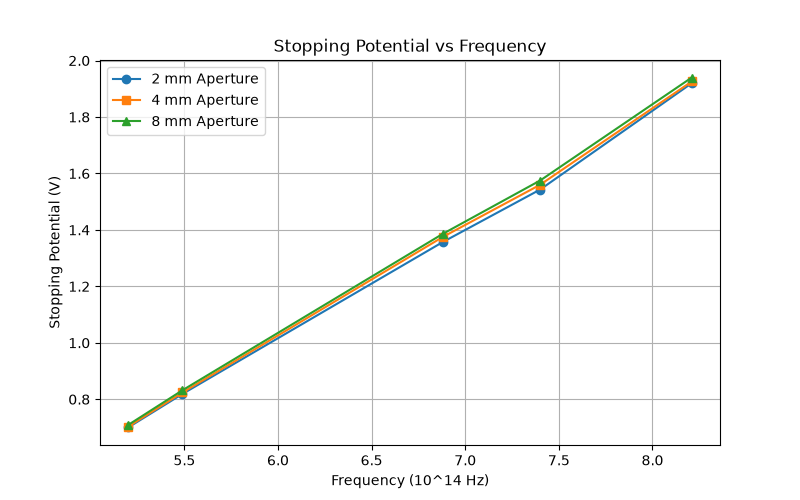
\includegraphics[width=0.8\textwidth]{graph1_vs_f.png}
    \caption{Stopping Potential versus Frequency for different aperture sizes. The slope of these linear fits is used to calculate Planck's constant.}
    \label{fig:graph1}
\end{figure}

\begin{figure}[H]
    \centering
    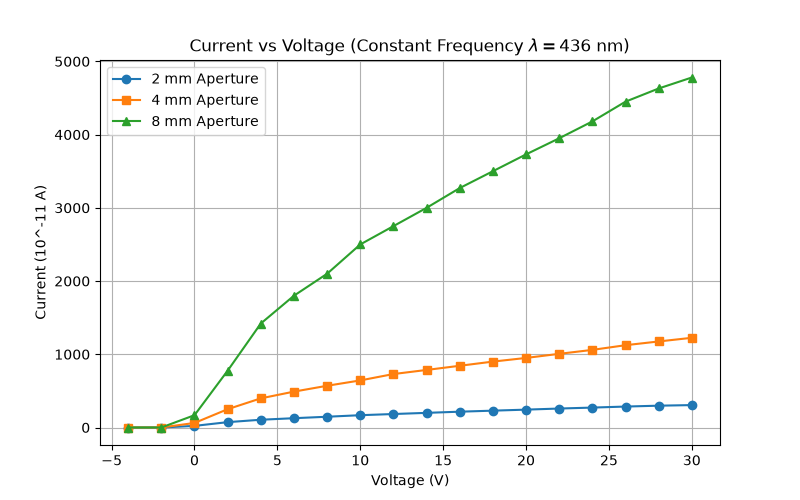
\includegraphics[width=0.8\textwidth]{graph2_i_vs_v_intensity.png}
    \caption{Current versus Voltage for varying light intensities (different apertures) at a constant frequency ($\lambda = 436$ nm). Note how the stopping potential remains constant across intensities.}
    \label{fig:graph2}
\end{figure}

\begin{figure}[H]
    \centering
    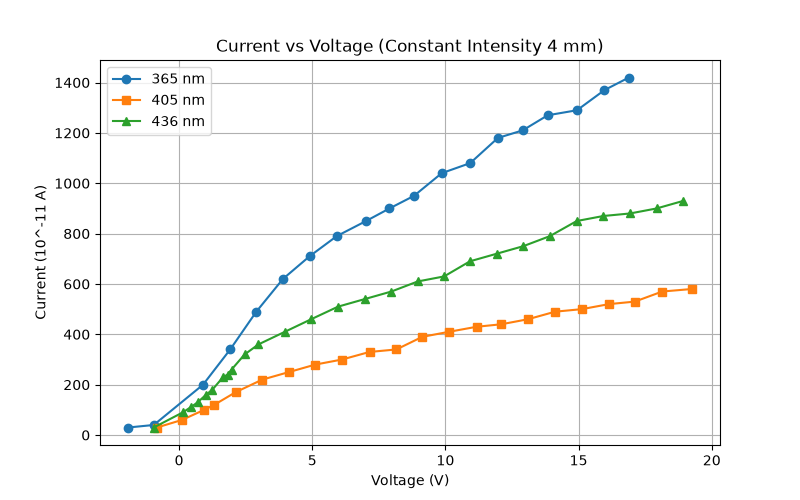
\includegraphics[width=0.8\textwidth]{graph3_i_vs_v_freq.png}
    \caption{Current versus Voltage for different frequencies at a constant intensity (4 mm aperture). The stopping potential becomes increasingly negative for higher frequencies.}
    \label{fig:graph3}
\end{figure}

\section{Error Calculation}
The accepted value of Planck's constant is $h_{accepted} = 6.626 \times 10^{-34}$ J$\cdot$s.

The percentage error in our experimental calculation is:
\begin{align*}
    \text{Percentage Error} &= \left| \frac{h_{experimental} - h_{accepted}}{h_{accepted}} \right| \times 100 \% \\
    &= \left| \frac{6.428 \times 10^{-34} - 6.626 \times 10^{-34}}{6.626 \times 10^{-34}} \right| \times 100 \% \\
    &= \left| \frac{-0.198}{6.626} \right| \times 100 \% \\
    &\approx 2.99 \%
\end{align*}

\section{Discussion}
In this experiment, we observed the fundamental properties of the photoelectric effect. The experiment confirmed that the stopping potential depends on the frequency of the incident light and is independent of its intensity. It also verified that the saturation current depends on the intensity of light but not its frequency. The linear relationship between stopping potential and frequency strongly supports the quantum theory of light.

In real life conditions, small discrepancies between the theoretical assumptions and experimental results can occur due to the reverse anode current and dark current of the cathode. These small currents can make it difficult to pinpoint the exact stopping potential where the true photocurrent is zero. Furthermore, external factors like stray light or instrument calibration could contribute to deviations from the ideal theoretical values, leading to the observed $2.99\%$ error in Planck's constant.

\section{References}
\begin{enumerate}
    \item Instruction Manual, Photoelectric Effect Apparatus, Model No. SE 6609, PASCO scientific.
    \item Halliday, D., Resnick, R., and Walker, J. Fundamentals of Physics.
\end{enumerate}

\section{Lab Observation}
The raw observation sheets from the laboratory experiment are attached below.

\begin{figure}[H]
    \centering
    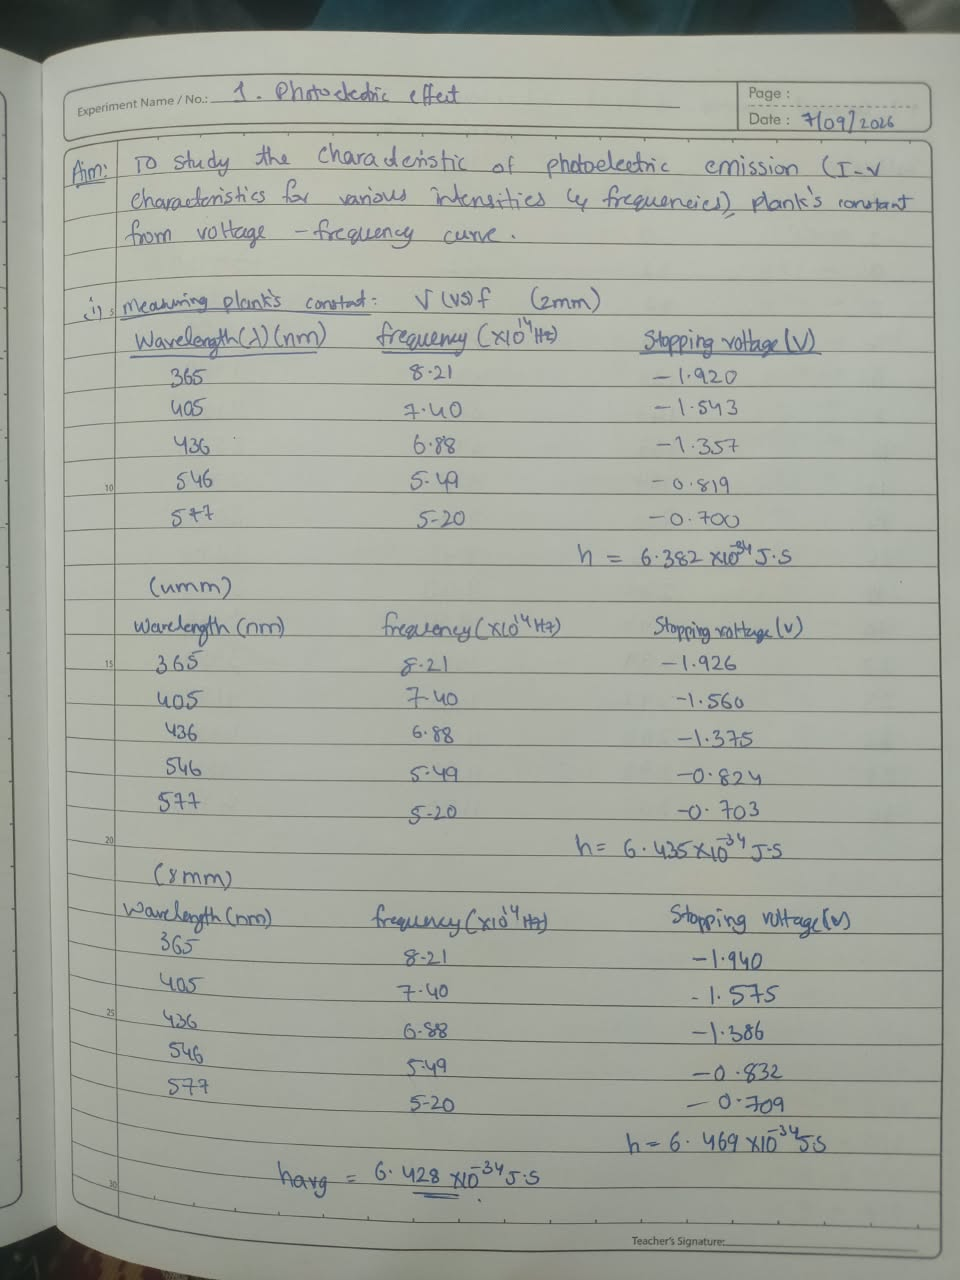
\includegraphics[width=0.8\textwidth]{../observations/WhatsApp Image 2026-10-05 at 11.12.44 PM.jpeg}
    \caption{Raw observation sheet 1: Measuring Planck's constant.}
\end{figure}

\begin{figure}[H]
    \centering
    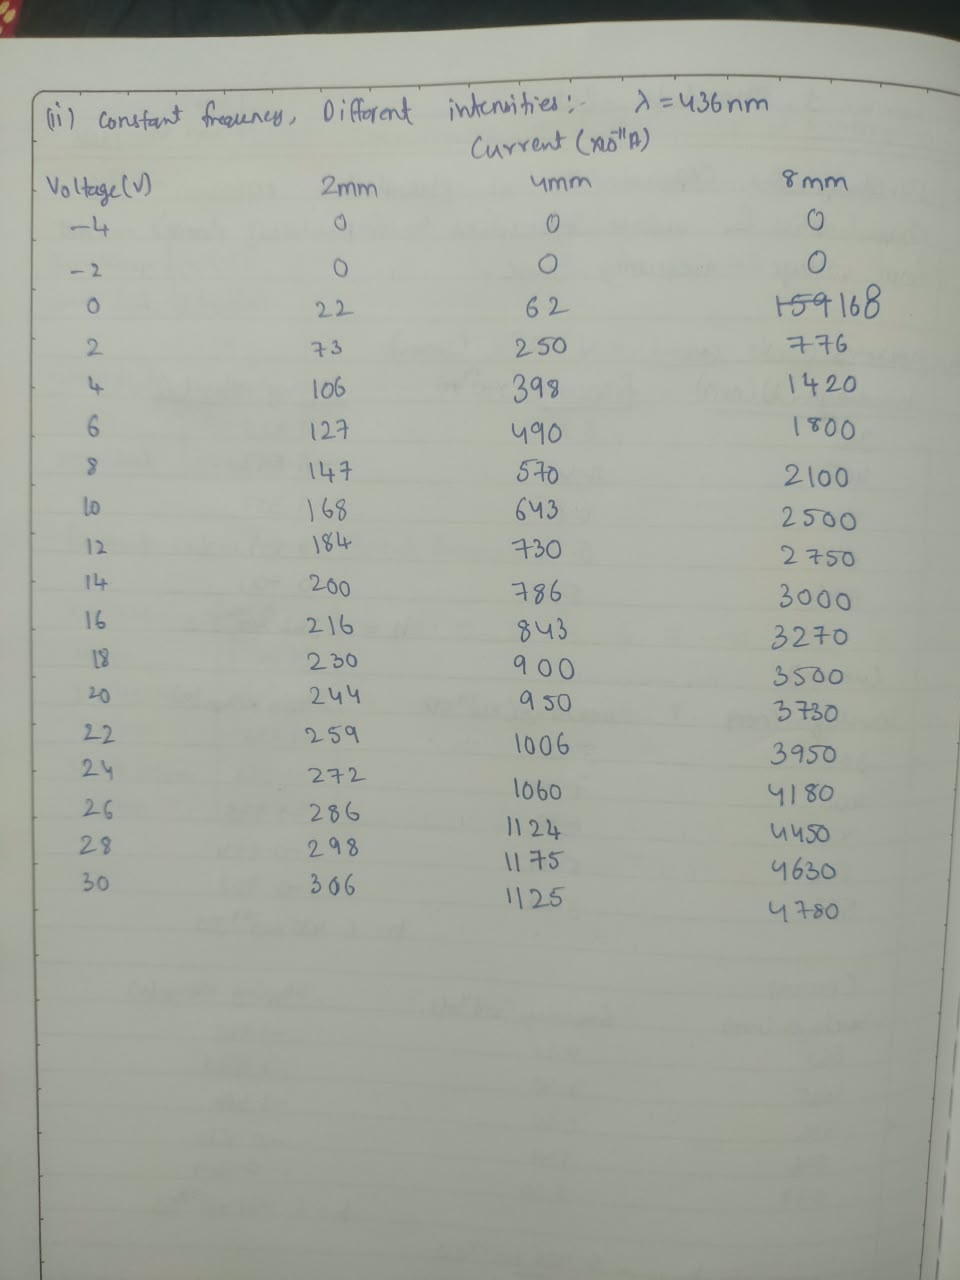
\includegraphics[width=0.8\textwidth]{../observations/WhatsApp Image 2026-10-05 at 11.12.45 PM.jpeg}
    \caption{Raw observation sheet 2: Constant frequency, different intensities.}
\end{figure}

\begin{figure}[H]
    \centering
    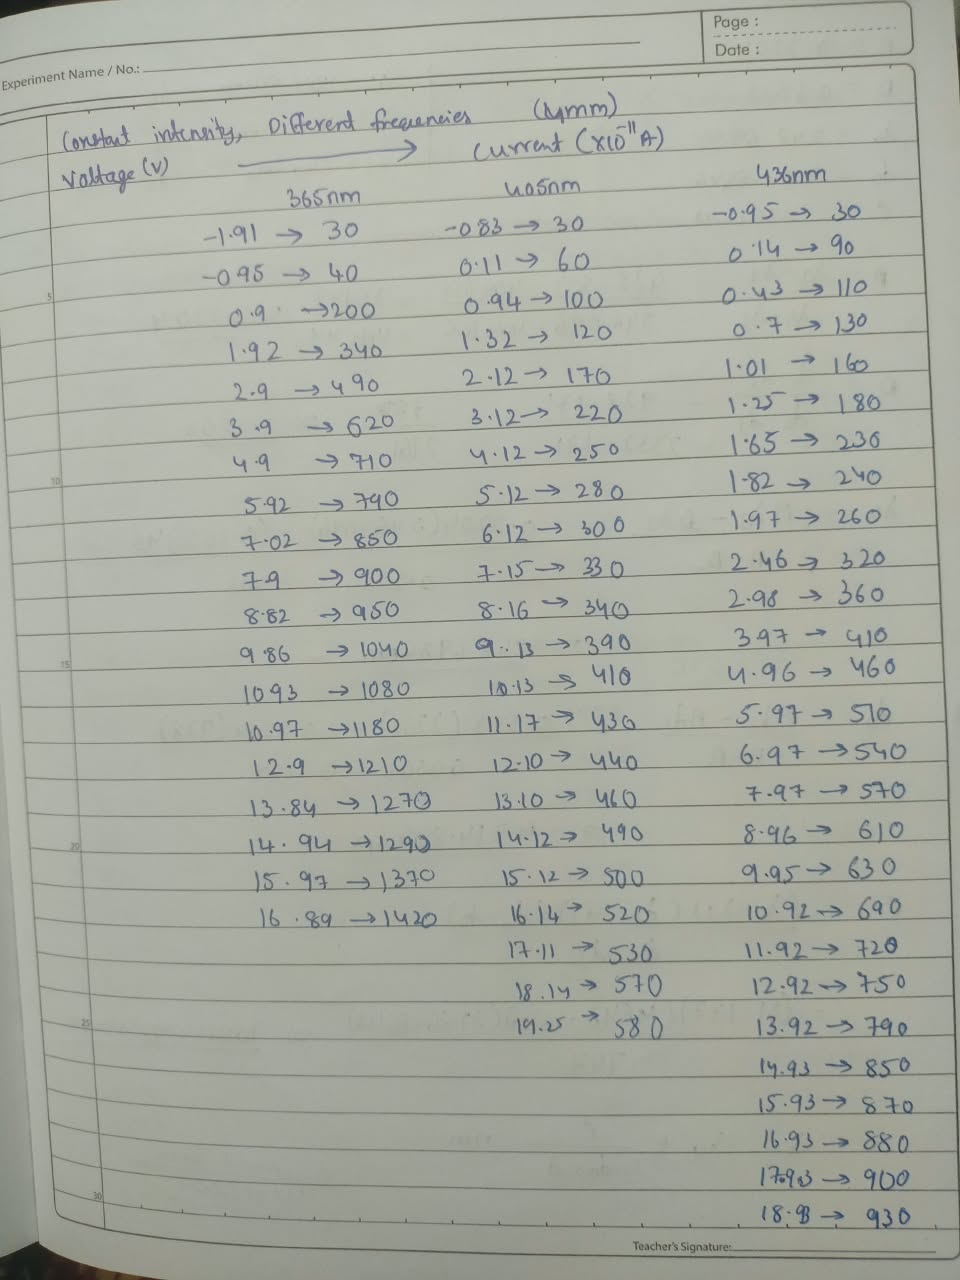
\includegraphics[width=0.8\textwidth]{../observations/WhatsApp Image 2026-10-05 at 11.12.46 PM.jpeg}
    \caption{Raw observation sheet 3: Constant intensity, different frequencies.}
\end{figure}

\end{document}
